\section{Results}

\subsection{Overall Capacity Comparison}

We first evaluated whether increasing backbone capacity within the ResNet family improves camera-trap generalization. Figure~\ref{fig:capacity-generalization} summarizes the in-domain and out-of-domain behavior of the ResNet capacity sweep across the three evaluation settings. Increasing backbone capacity generally improved performance, but the improvement was not sufficient to remove the generalization gap. In the cross-location and day-to-night settings, ResNet-101 achieved the strongest OOD performance among the tested backbones, while in the night-to-day setting ResNet-50 was the strongest model in the initial capacity comparison. This pattern suggests that larger backbones provide useful representational capacity, but capacity alone does not solve the domain shift problem.

\begin{figure}[h]
    \centering
    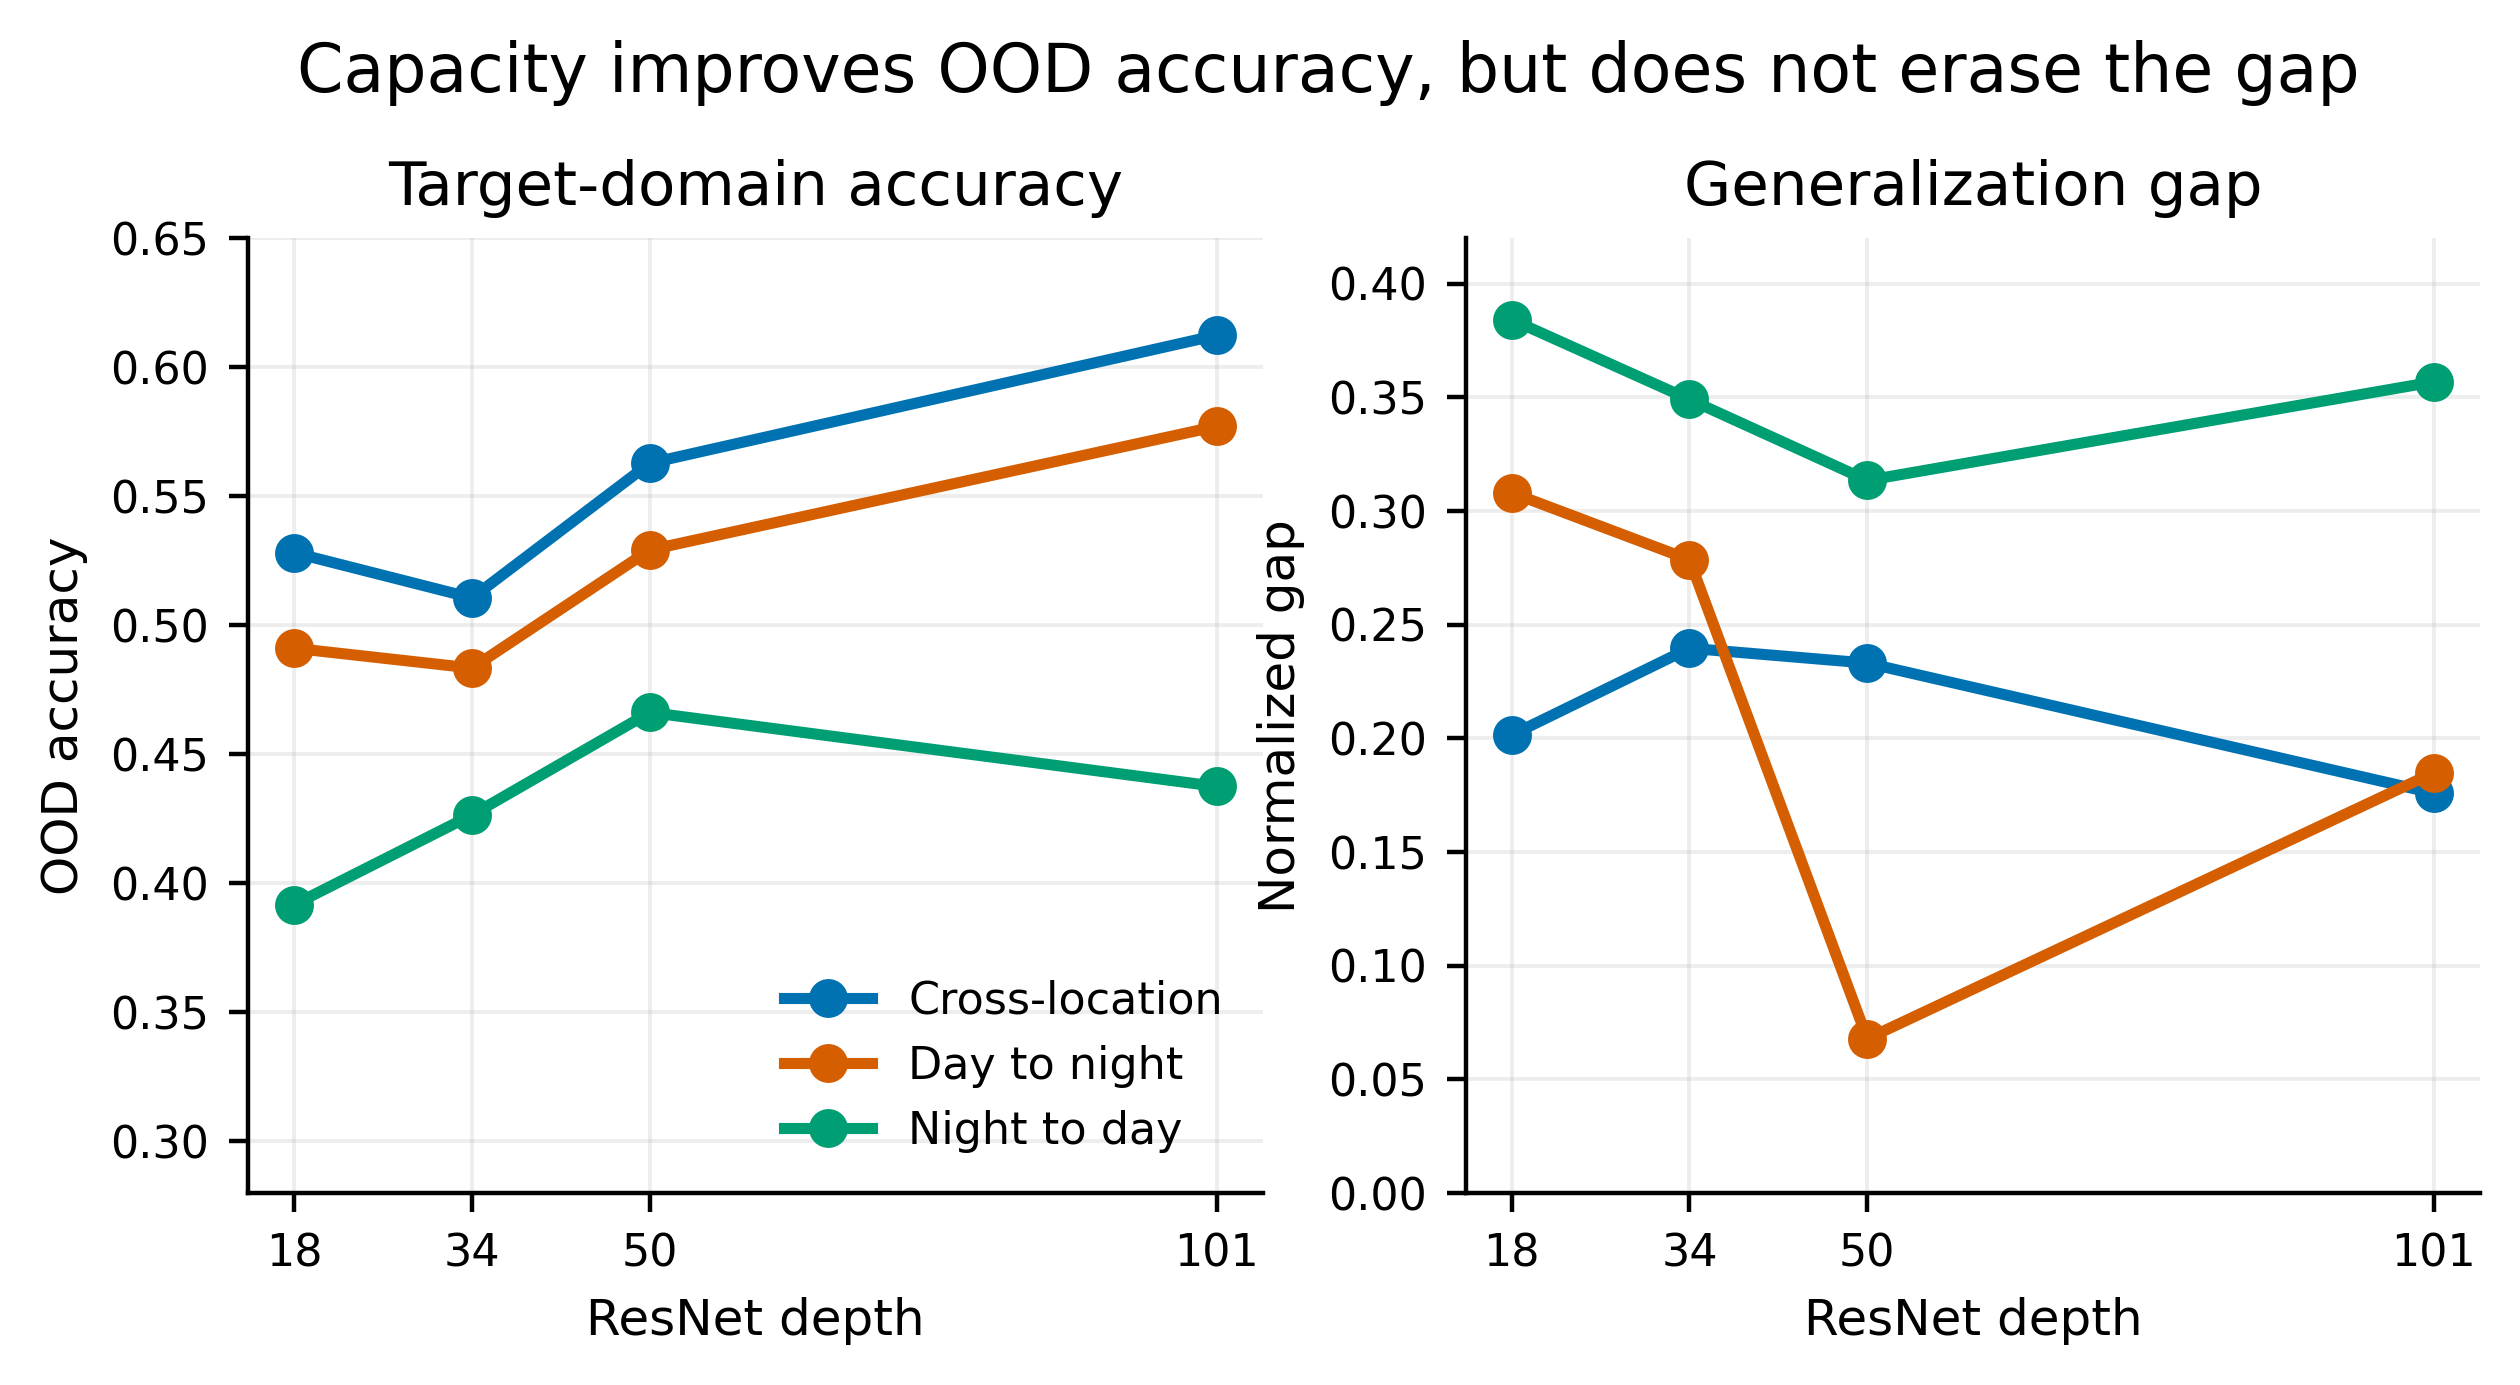
\includegraphics[width=\linewidth]{figures/figure1_capacity_generalization.png}
    \caption{\textbf{Capacity comparison across domain shifts.} ResNet-18, ResNet-34, ResNet-50, and ResNet-101 were evaluated on cross-location, day-to-night, and night-to-day transfer. Larger backbones improve some settings, but the OOD gap remains.}
    \label{fig:capacity-generalization}
\end{figure}

This result is important because the ResNet-family sweep changes more than depth alone: the backbones differ in residual block type, feature dimensionality, and computational cost. Therefore, the experiment should be interpreted as a practical backbone-capacity comparison rather than a causal isolation of depth. The key takeaway is that a stronger backbone improves the baseline but does not remove the need to understand the source of OOD failure.

\subsection{Out-of-Domain Generalization Gap}

We next analyzed the gap between in-domain and out-of-domain target splits. Across all three scenarios, models performed better on in-domain target splits than on shifted target splits, confirming that the dataset design creates meaningful domain shift. The normalized gap was used to compare transfer degradation across scenarios with different in-domain accuracies:

\[
\mathrm{Normalized\ Gap}
=
\frac{
\mathrm{Accuracy}_{\mathrm{ID}}
-
\mathrm{Accuracy}_{\mathrm{OOD}}
}{
\mathrm{Accuracy}_{\mathrm{ID}}
}.
\]

The capacity baseline shows that the gap persists even when using larger ImageNet-pretrained ResNet backbones. For example, the best initial capacity results reached approximately \(0.612\) OOD accuracy with ResNet-101 in the cross-location setting, \(0.577\) OOD accuracy with ResNet-101 in the day-to-night setting, and \(0.466\) OOD accuracy with ResNet-50 in the night-to-day setting. However, the remaining normalized gaps show that model capacity alone does not provide robust transfer.

This motivates the hypothesis-driven intervention results below. If the gap were mainly caused by simple appearance mismatch, then brightness or visibility interventions should reduce it. If it were mainly caused by background shortcuts, then background suppression or background-only diagnostics should explain the model behavior. If the gap were caused by unstable nuisance cues, then perturbation-based diversification should help. Finally, if the bottleneck were object localization and framing, object-centric diagnostics should provide the strongest improvement.

\subsection{Class-Level Error Analysis}

Aggregate accuracy hides substantial class-level variation, so we analyzed per-class F1 scores and confusion matrices. Figure~\ref{fig:class-failures} summarizes class imbalance and failure modes. Rare and visually difficult classes, especially rodent, remained challenging across the hardest target splits. This indicates that OOD failure is not only a global accuracy problem but also a class-specific robustness problem.

\begin{figure}[h]
    \centering
    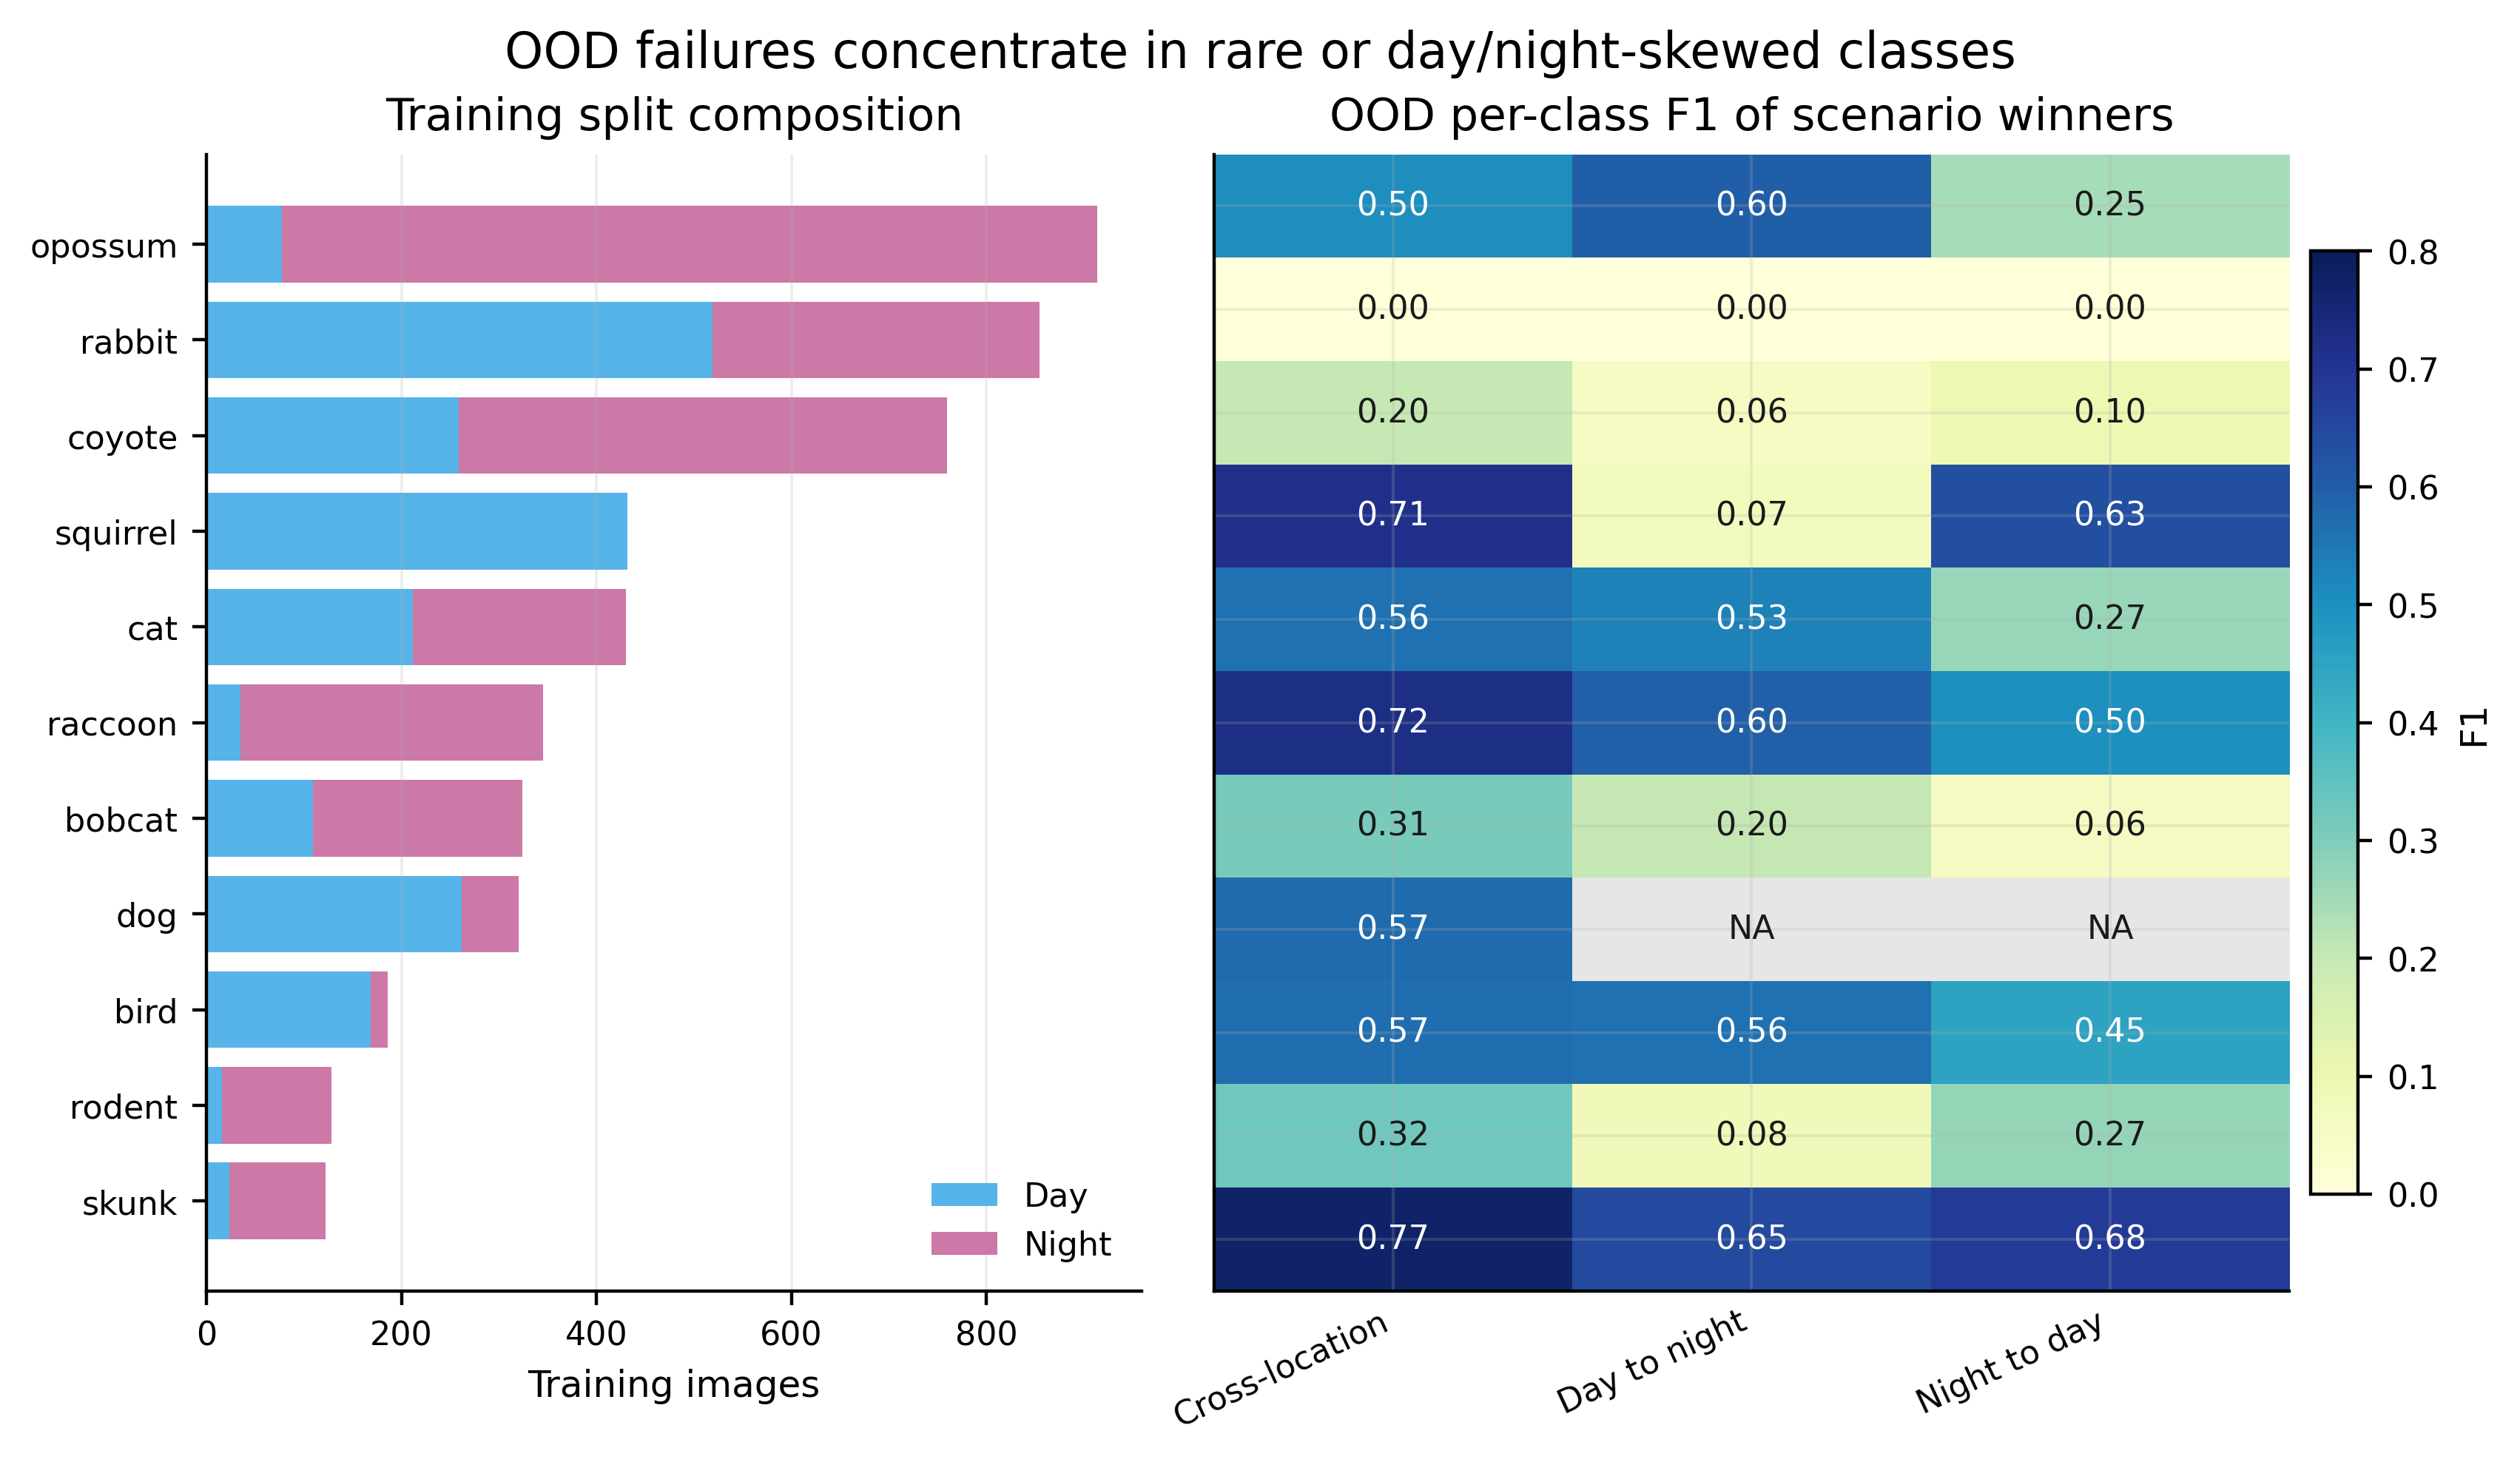
\includegraphics[width=\linewidth]{figures/figureS1_class_imbalance_and_failure_modes.png}
    \caption{\textbf{Class imbalance and target-split failure modes.} Per-class support and F1 scores show that aggregate accuracy can hide severe failures on rare or visually difficult classes. Rodent is consistently difficult, suggesting a separate small-object, data-scarcity, or label-ambiguity problem.}
    \label{fig:class-failures}
\end{figure}

The object-centric per-class analysis in Figure~\ref{fig:object-crop-class-delta} further clarifies which classes benefit from localization. Object crops substantially improved several visually confusable or context-sensitive classes, including rabbit, bird, bobcat, opossum, cat, and coyote in at least some target settings. However, rodent remained near failure even after object cropping, suggesting that not all errors are explained by background context. Some failures likely arise from small object size, insufficient training support, low image quality, or label ambiguity.

\begin{figure}[h]
    \centering
    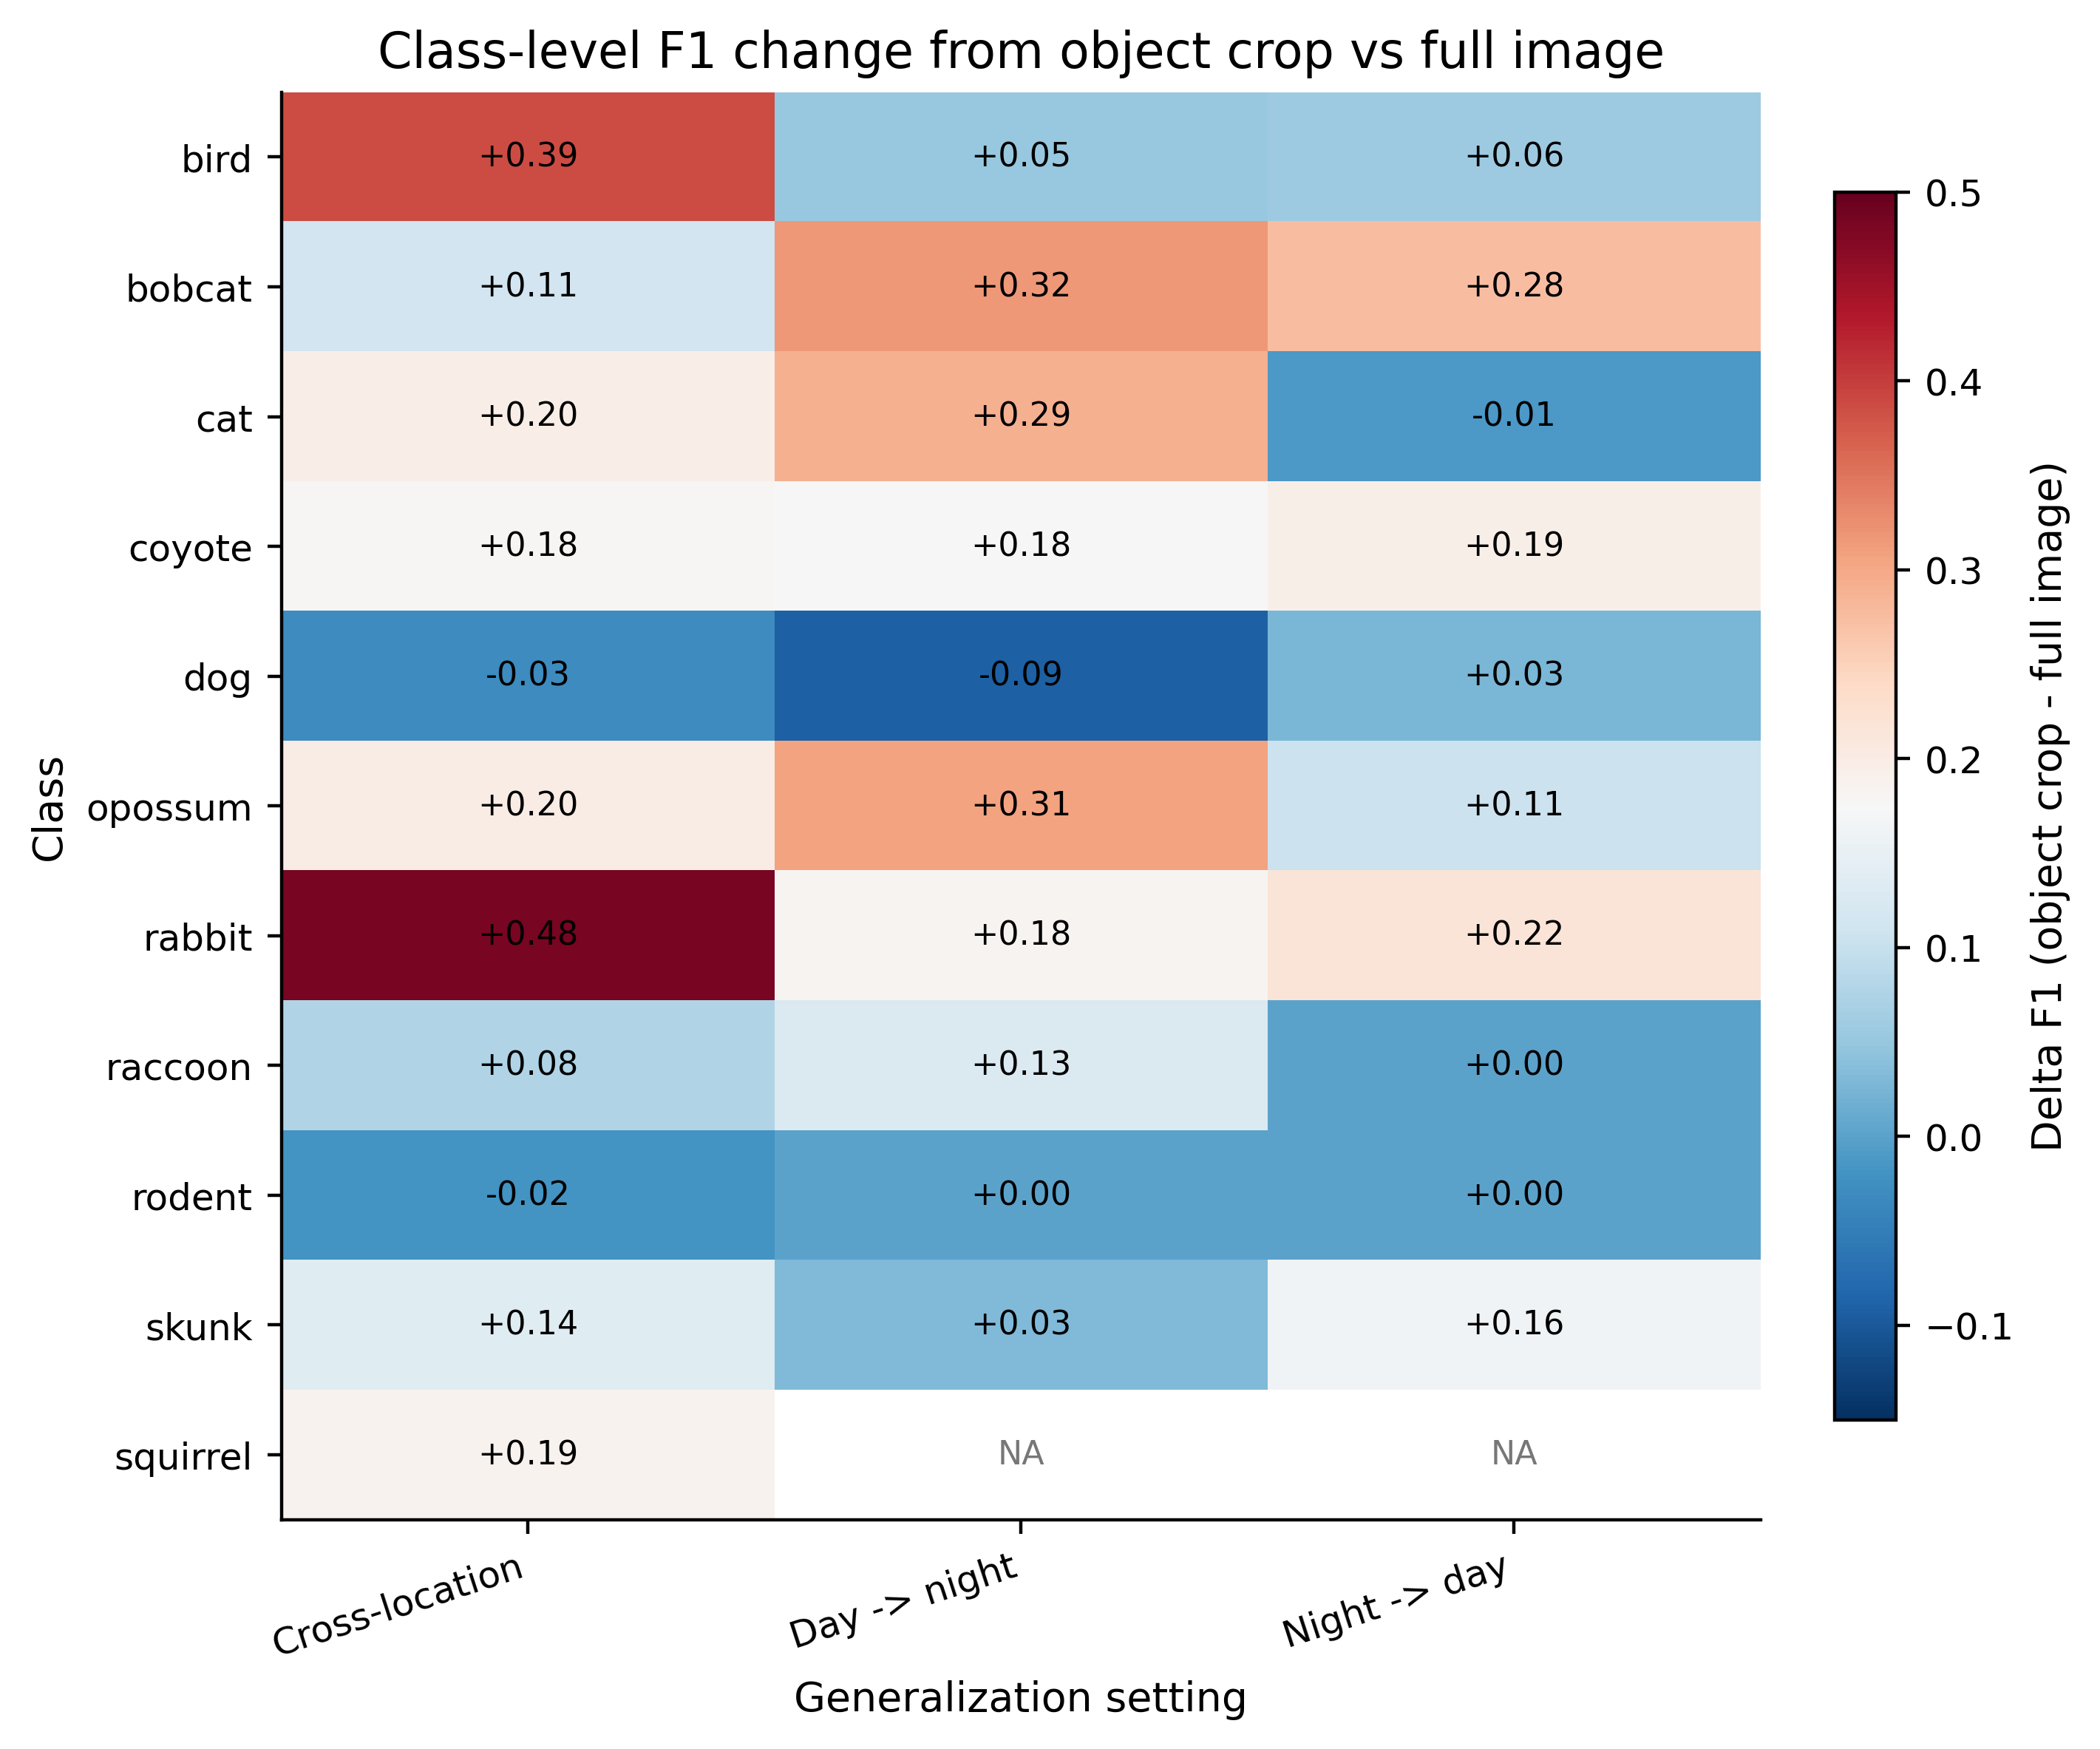
\includegraphics[width=\linewidth]{figures/figure5_object_crop_per_class_delta.png}
    \caption{\textbf{Class-level F1 change from object cropping.} Each cell shows the change in target-split F1 after replacing the full image with an oracle object crop. Object crops improve many classes but do not solve all rare-class failures.}
    \label{fig:object-crop-class-delta}
\end{figure}

This error analysis supports the main interpretation of the project: the dominant failure mode is not simply class imbalance or low model capacity. Object localization helps many classes, but some classes require additional treatment beyond the interventions tested here.

\subsection{Intervention Results}

We organized the intervention experiments around competing explanations for OOD failure. The first set of interventions tested whether reducing nuisance information or aligning appearance distributions improves transfer. Figure~\ref{fig:train-intervention-deltas} shows that these train-time interventions were generally weak or negative. Nuisance-reduction interventions had a negative mean OOD effect in the initial comparison, and only a small fraction of cells improved over the original baseline. This suggests that simply removing or suppressing nuisance cues can also remove useful ecological context or introduce train-test mismatch.

\begin{figure}[h]
    \centering
    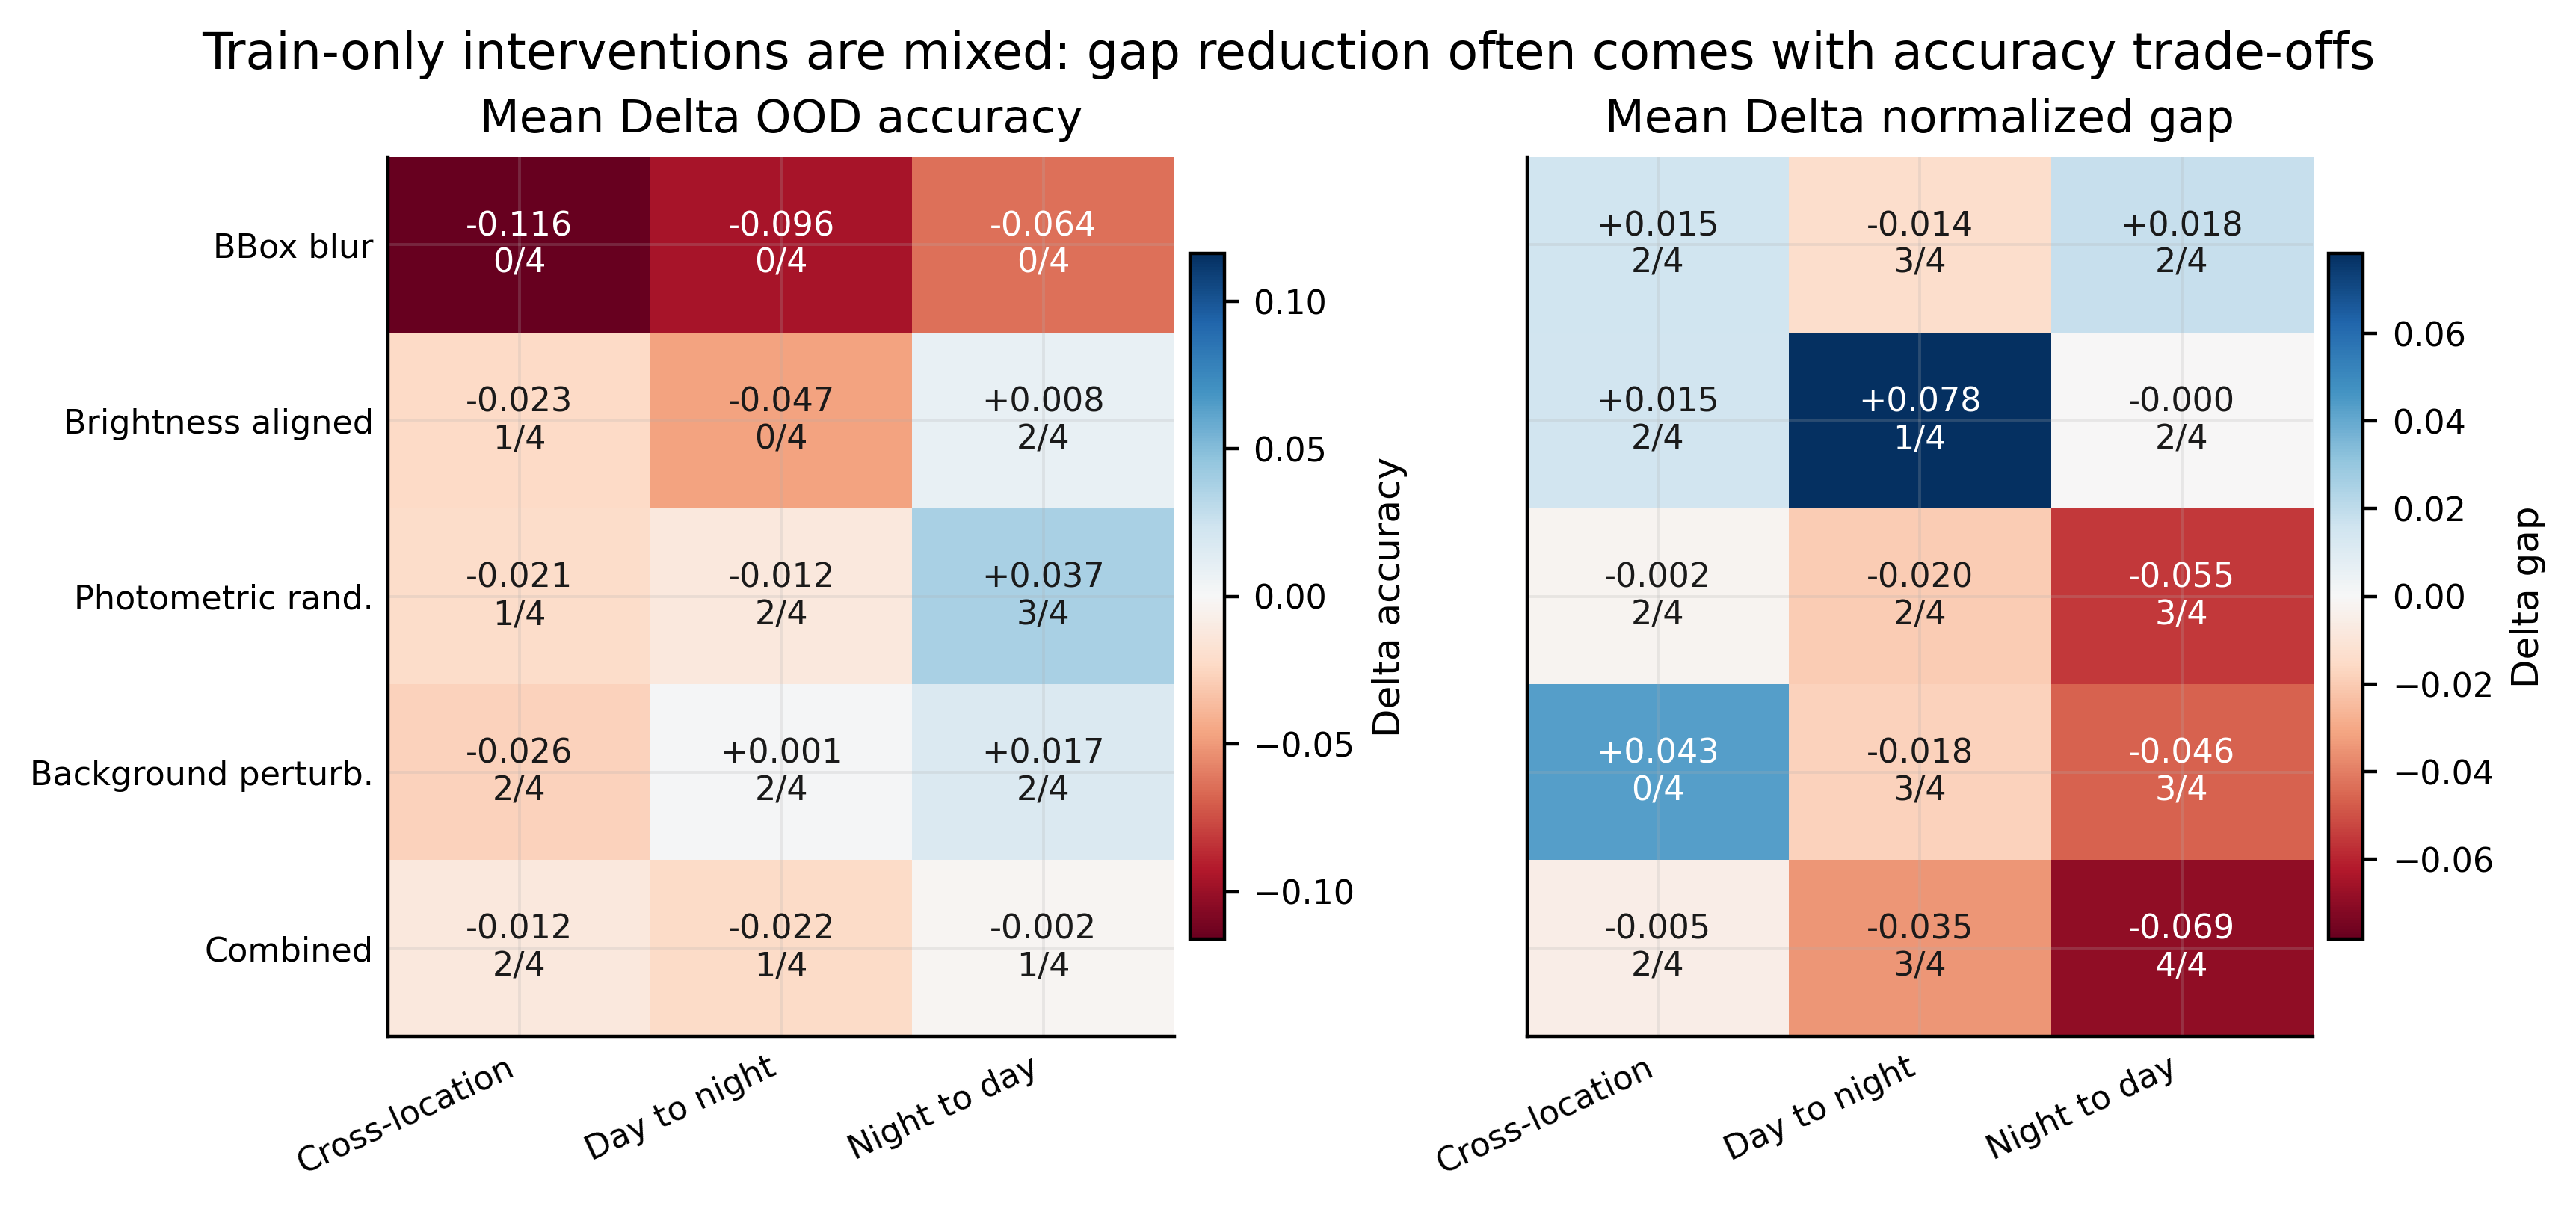
\includegraphics[width=\linewidth]{figures/figure2_train_time_intervention_deltas.png}
    \caption{\textbf{Train-time intervention effects.} Changes in OOD accuracy and normalized gap are shown for nuisance-reduction and perturbation-style interventions. Most effects are weak, mixed, or negative, indicating that simple image-level interventions do not reliably solve camera-trap OOD generalization.}
    \label{fig:train-intervention-deltas}
\end{figure}

The visibility/detail interventions provide a similarly nuanced result. Figure~\ref{fig:visibility-effects} shows that test-only visibility enhancement often hurts performance, while train-test consistent enhancement provides only small average gains. This supports the interpretation that post-hoc enhancement can create distribution mismatch, and that low-light visibility is not the only explanation for cross-time transfer failure.

\begin{figure}[h]
    \centering
    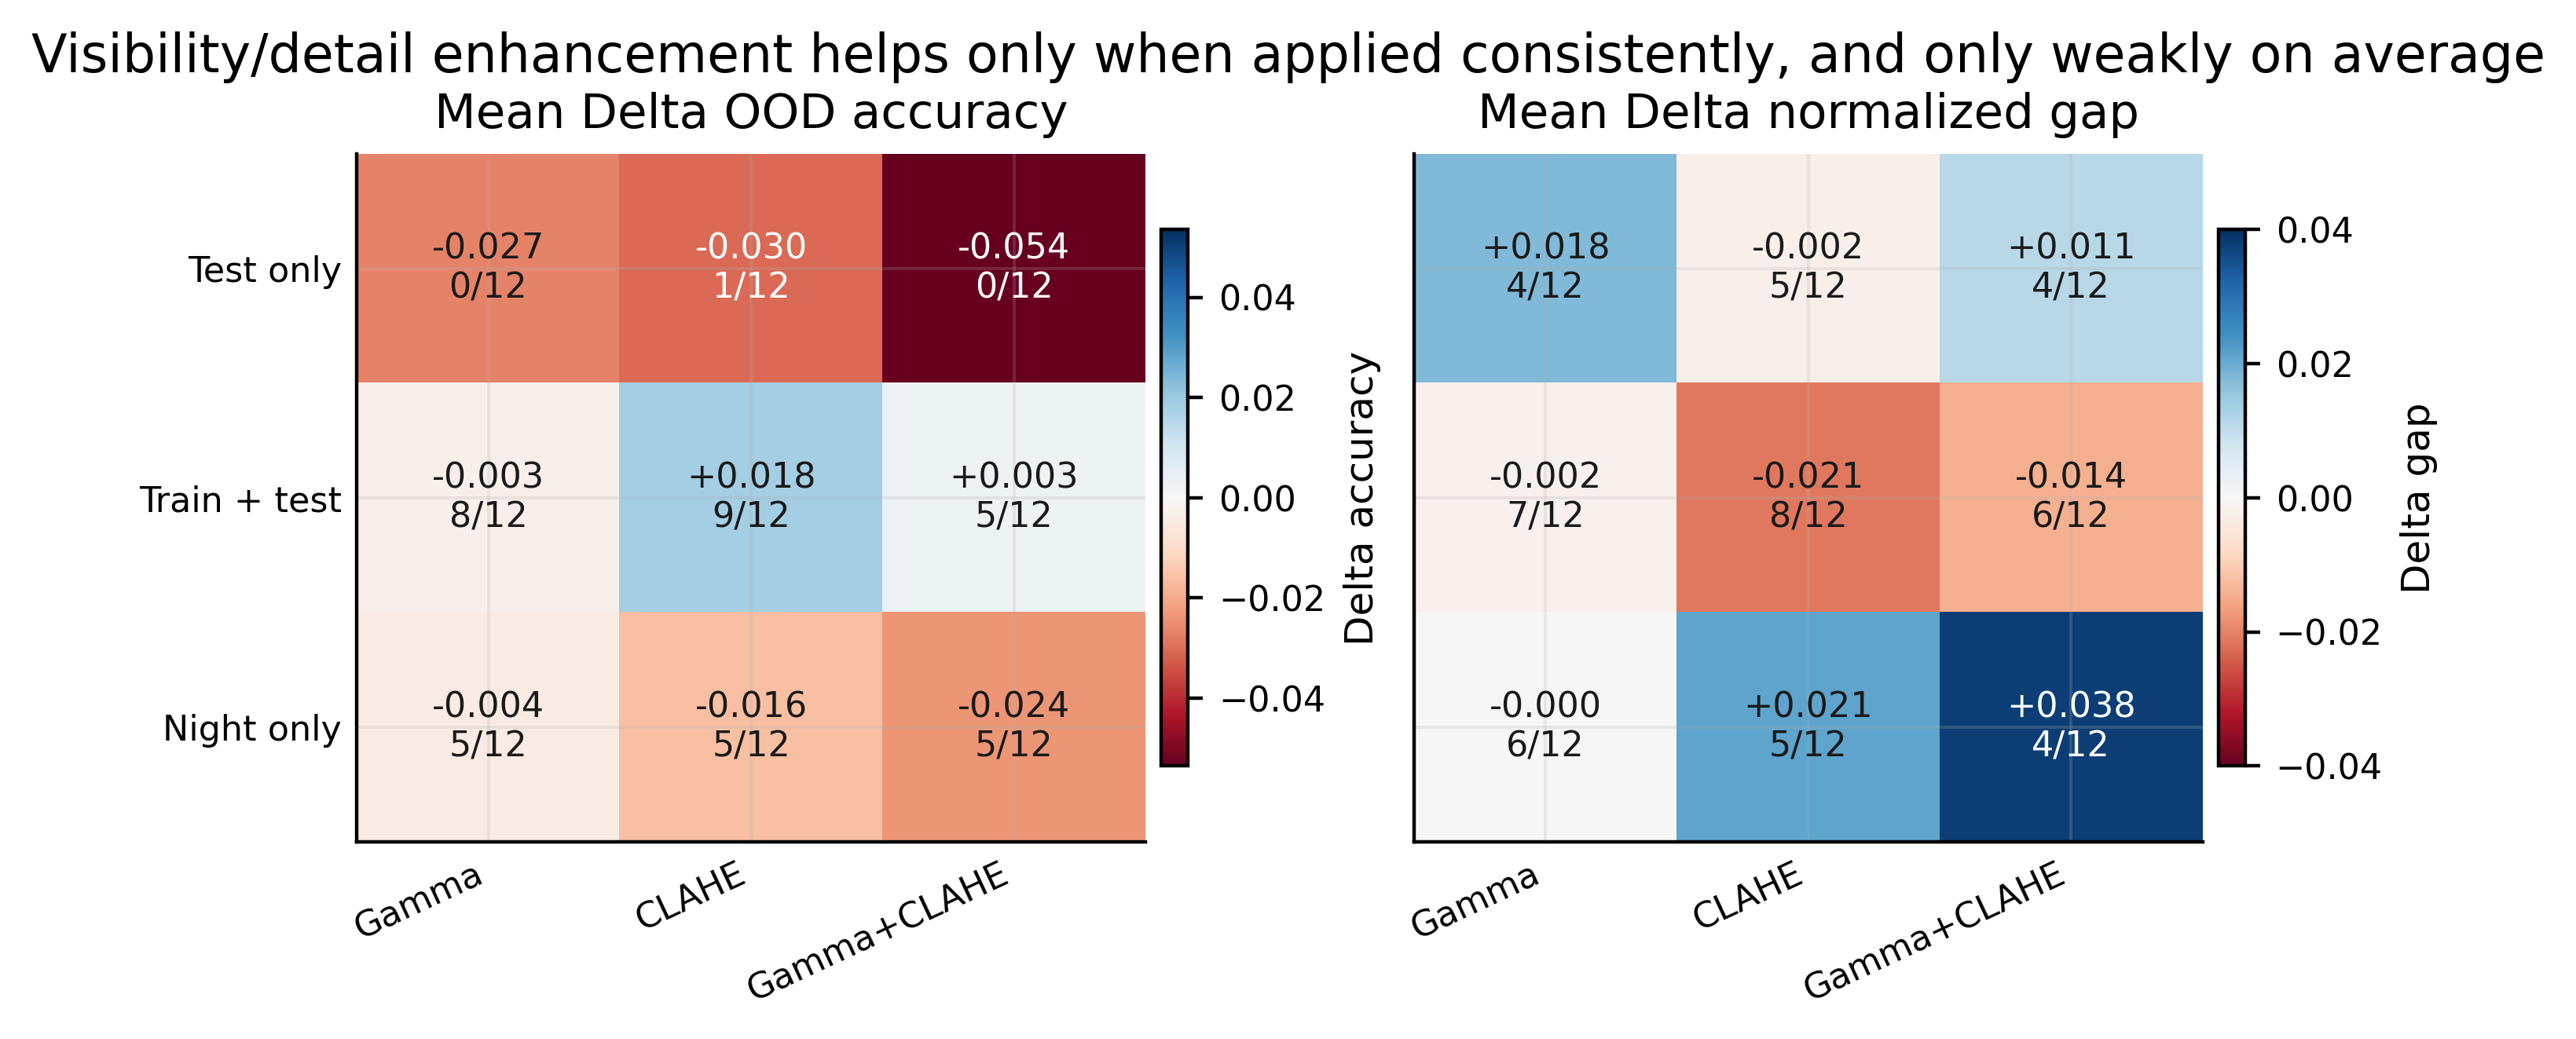
\includegraphics[width=\linewidth]{figures/figure3_visibility_detail_effects.png}
    \caption{\textbf{Visibility and detail enhancement effects.} Gamma correction, CLAHE, and gamma+CLAHE were evaluated under different preprocessing scopes. Test-only enhancement is often harmful, while train-test consistent enhancement provides limited gains.}
    \label{fig:visibility-effects}
\end{figure}

The strongest intervention result came from the object-centric diagnostic experiments. Figure~\ref{fig:object-centric-diagnostic} compares the full-image baseline, background-only, foreground-only, and object-crop views. Background-only performed poorly, indicating that background alone is not sufficient for robust classification. Foreground-only was mixed, suggesting that removing background is not enough by itself. In contrast, object crops produced the largest and most consistent gains across the three domain shifts.

\begin{figure}[h]
    \centering
    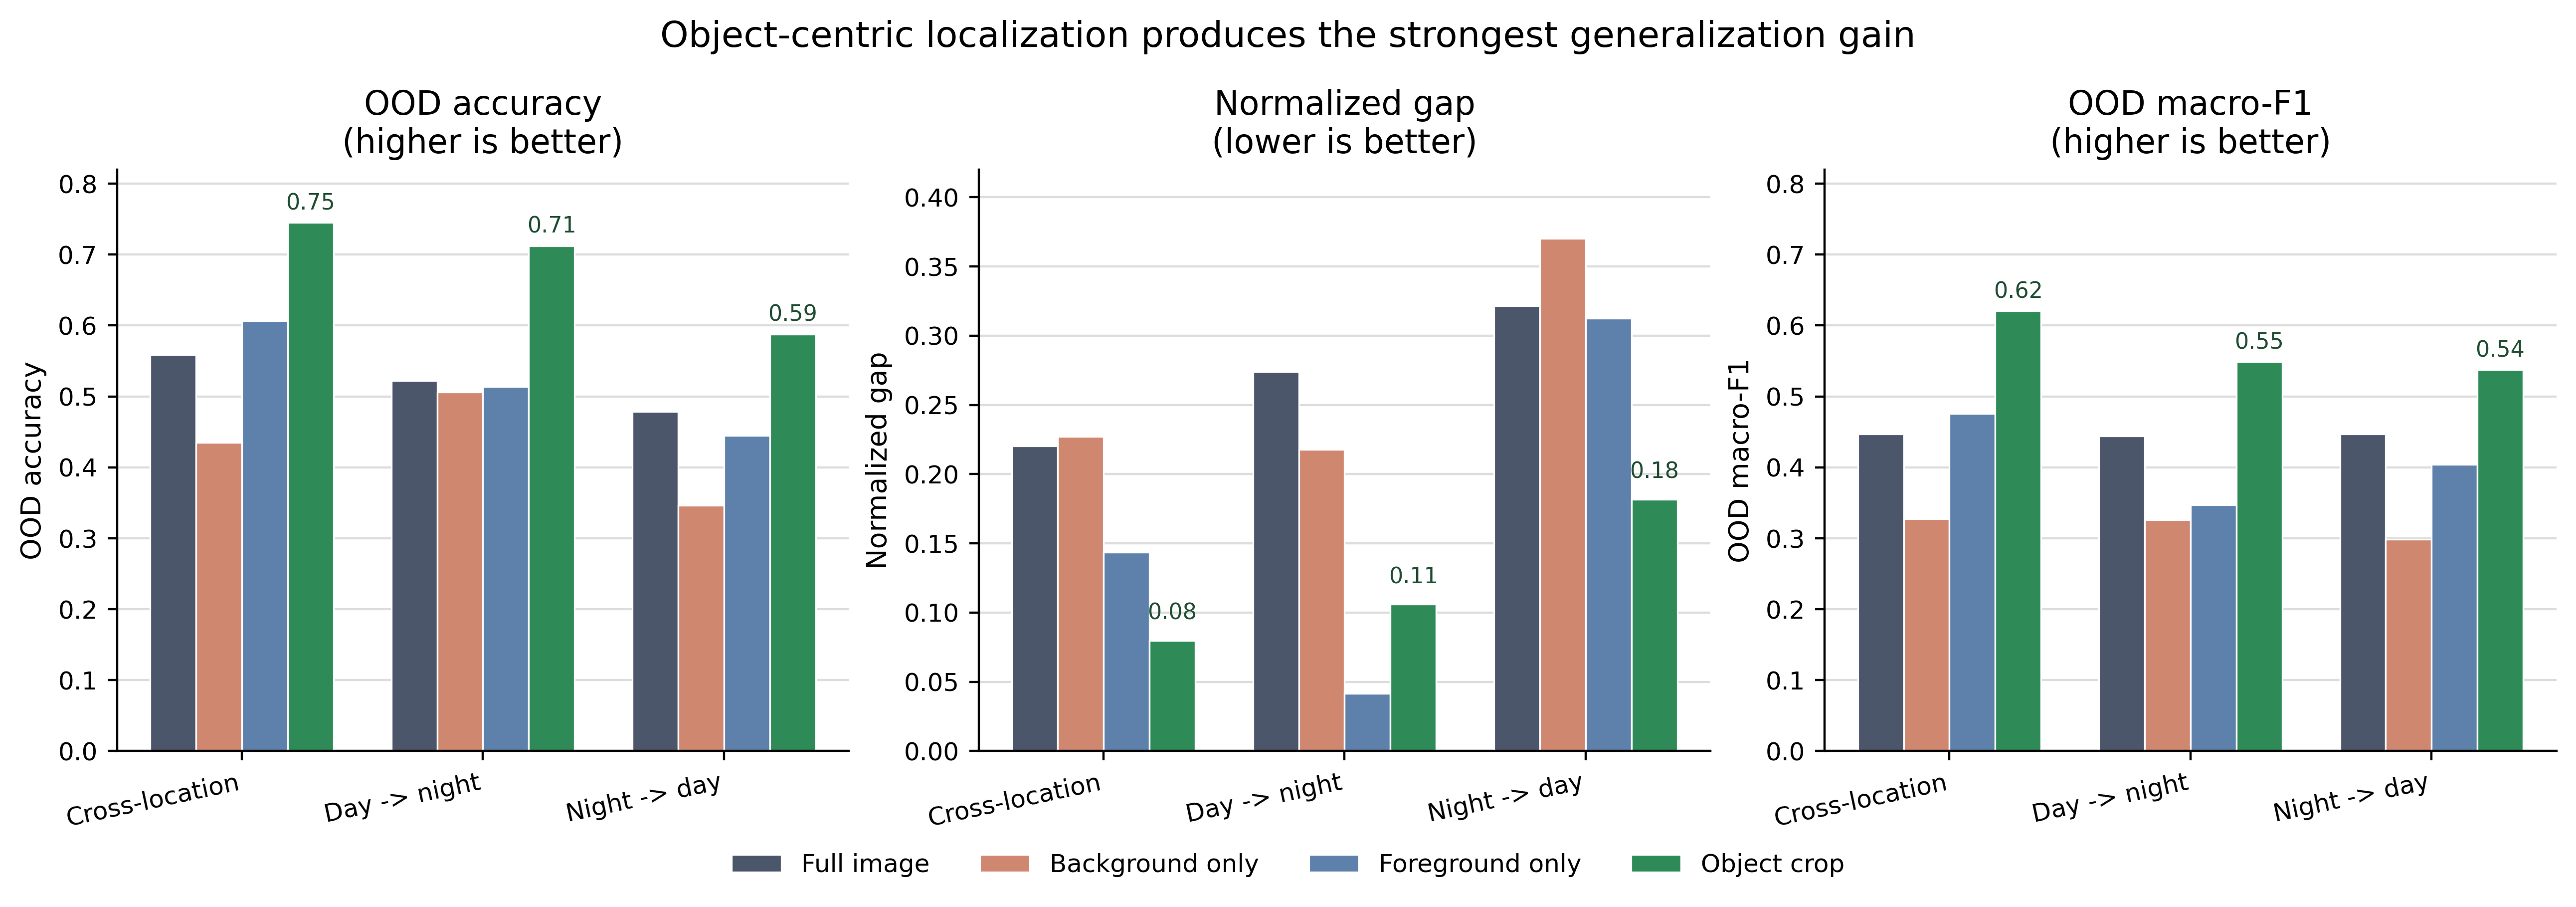
\includegraphics[width=\linewidth]{figures/figure4_object_centric_diagnostic.png}
    \caption{\textbf{Object-centric diagnostic results.} Full-image, background-only, foreground-only, and object-crop views were compared across the main transfer settings. Object crops produced the strongest gains in OOD accuracy and macro-F1 while reducing normalized gaps.}
    \label{fig:object-centric-diagnostic}
\end{figure}

Using the seed-matched full-image baseline, object crops improved OOD accuracy from \(0.559\) to \(0.745\) in cross-location transfer, from \(0.522\) to \(0.713\) in day-to-night transfer, and from \(0.479\) to \(0.588\) in night-to-day transfer. These correspond to gains of \(+18.6\), \(+19.0\), and \(+10.9\) percentage points, respectively. OOD macro-F1 also improved in all three scenarios. These results indicate that the most useful diagnostic intervention is not a global image transformation but an oracle object-centered view.

Finally, Figure~\ref{fig:loss-followups} summarizes the rare-class and loss follow-ups. Removing class weights, using a class-balanced sampler, and using focal loss produced mixed results and did not match the object-crop gains. This suggests that class imbalance contributes to the difficulty of the task, but it does not fully explain the observed OOD generalization failures.

\begin{figure}[h]
    \centering
    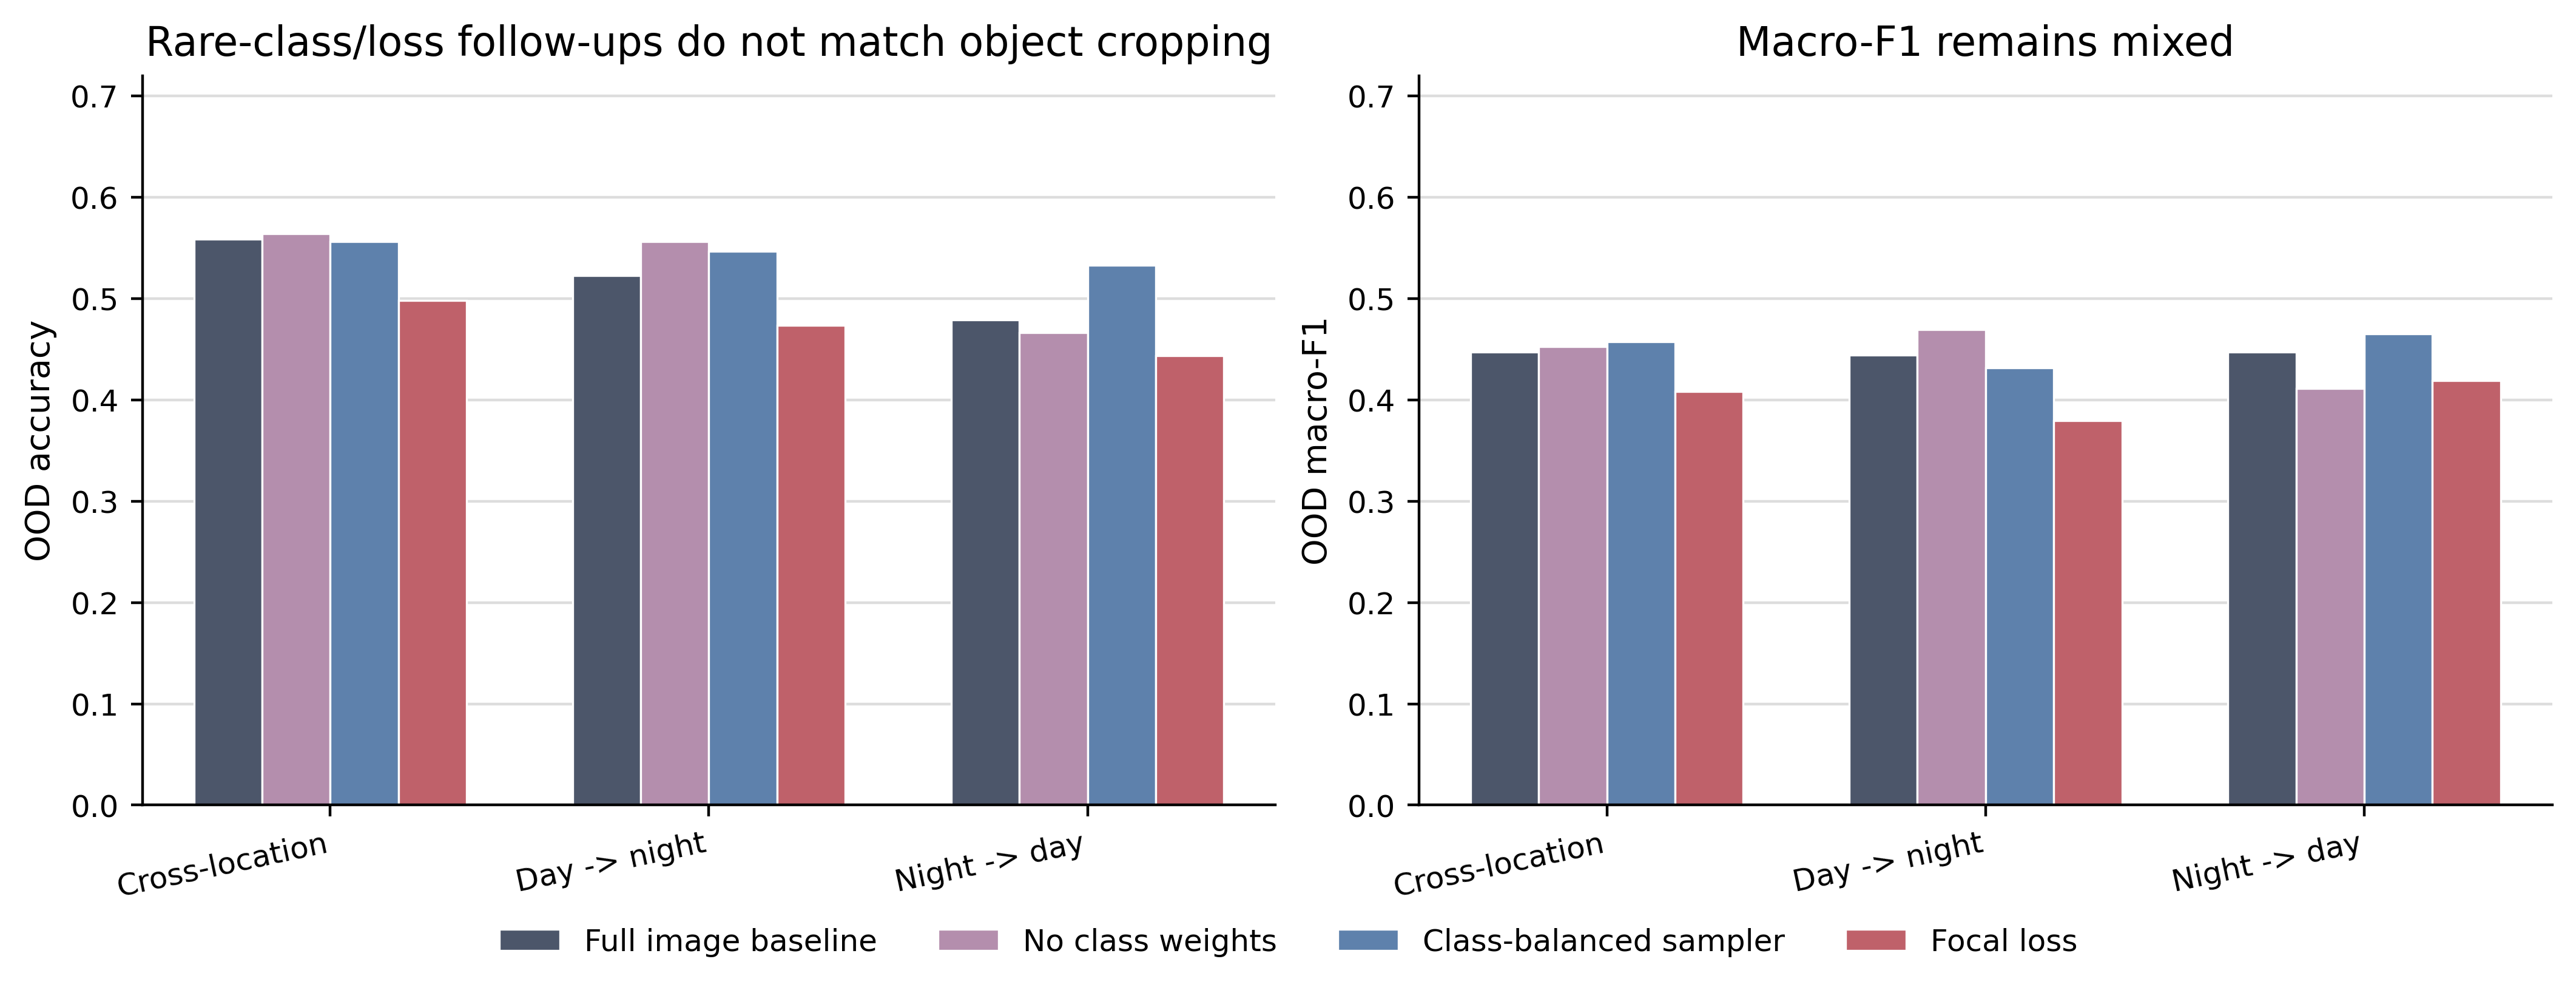
\includegraphics[width=\linewidth]{figures/figureS2_class_balance_loss_followups.png}
    \caption{\textbf{Rare-class and loss follow-up experiments.} No class weights, class-balanced sampling, and focal loss produced mixed effects. These follow-ups suggest that poor OOD macro-F1 is not explained by class imbalance alone.}
    \label{fig:loss-followups}
\end{figure}

Overall, the intervention results support a question-driven interpretation. Appearance mismatch, background reliance, and nuisance instability each explain part of the problem, but none of the corresponding global interventions consistently solved the gap. The strongest evidence points to object localization and framing: when the model receives an oracle object-centered crop, transfer improves sharply. Thus, camera-trap generalization appears to be limited more by object localization and context entanglement than by backbone capacity or global preprocessing alone.
